\documentclass[11pt]{article}

\usepackage[margin=1in]{geometry}
\usepackage{amsmath,amssymb}
\usepackage{booktabs}
\usepackage{array}
\usepackage{graphicx}
\usepackage{float}
\usepackage{hyperref}

\hypersetup{
  colorlinks=true,
  linkcolor=black,
  citecolor=black,
  urlcolor=blue
}

\title{Oracle-Anchored Fee-and-Width Control for LVR-Resilient Uniswap v4 Pools\\
\large A hook-level design note with analytic derivations, real-data validation, and a Dutch-auction repricing counterfactual}
\author{Mitchell Marfinetz\\
\href{mailto:mitchell.marfientz@nethermind.io}{mitchell.marfientz@nethermind.io}
\and
Joel Kahil\\
\href{mailto:joel@nethermind.io}{joel@nethermind.io}}
\date{April 2026}

\begin{document}
\maketitle

\begin{abstract}
Loss-versus-rebalancing (LVR) is the adverse-selection cost paid by automated market maker liquidity providers when pools quote stale prices relative to faster external markets. We study a concrete Uniswap v4 hook design that targets two levers implied by the LVR literature: toxic-flow pricing and marginal-liquidity shape. For a constant-product repricing event with oracle-pool log gap $z$, the exact fee on the toxic input needed to recapture the one-step stale-price loss is
\[
  f^\star(z) = e^{|z|/2} - 1,
\]
with local approximation $f^\star(z) \approx |z|/2$. For a centered concentrated-liquidity range of total log-width $W$, normalized gross LVR is amplified by $1/(1-e^{-W/4})$, yielding a minimum-width guard for any target latency budget.

The fee identity is validated on frozen real replay data: across 44 replay-clean windows containing 7,019 swaps, the exact replay fee-identity residual is at most $10^{-64}$. We also evaluate an auctioned repricing counterfactual on the saved October 10, 2025 oracle-fail stress day and on a checkpointed October 2025 month run across WETH/USDC, WBTC/USDC, LINK/WETH, and UNI/WETH. The month run completed 124 of 124 planned windows, covering 89,220 swap samples and 8,784 oracle updates. A 5,208-row USD-floor launch-policy sweep shows that immediate launch rules maintain 100\% clear rates in the counterfactual replay. A \$0.50 stale-loss floor is approximately 0.50 USDC for USDC-quoted pools but only about 0.000124 WETH for WETH-quoted pools, avoiding the under-triggering caused by a universal native-quote floor.

A 24-hour four-pool rerun over blocks 23,543,615 to 23,550,763 remains the main stress-day exhibit: the auctioned policy preserves immediate repricing while recapturing most toxic-flow LVR, whereas pure hook-only protection prevents realized toxic trades mostly by leaving pools stale. The current Solidity hook is hook-only: it uses \texttt{beforeSwap} for oracle-anchored fee overrides and \texttt{beforeAddLiquidity} for width and centering guards. The auction is a counterfactual execution policy and proposed module/relay path, not a deployed on-chain branch. The paper's claim is therefore split deliberately: fee accounting is validated on frozen real data; auctioned repricing has historical counterfactual support under adversarial repricing; mixed-flow market quality is measured for the hook replay path; and production auction deployment remains outside this draft.
\end{abstract}

\section{Introduction}

Automated market makers quote from on-chain state. When a reference market moves first, informed flow can trade against the stale pool until the AMM is repriced. The profit of that informed repricing trade comes from liquidity providers (LPs). The LVR framework of Milionis, Moallemi, Roughgarden, and Zhang formalizes this cost as the difference between the AMM LP's performance and a self-financing rebalancing strategy that holds the same inventory but trades continuously at external prices \cite{milionis-lvr}.

This gives a clean hook-level design target. If LVR is driven by volatility, stale prices, and marginal liquidity, then a low-LVR Uniswap v4 pool should control three things:

\begin{enumerate}
  \item toxic-flow pricing when the pool is stale relative to a trusted reference;
  \item admission of overly narrow or off-center concentrated-liquidity positions;
  \item the execution path for repricing, so protection does not simply make the pool stale.
\end{enumerate}

Uniswap v4 hooks make these controls programmable at the pool boundary \cite{uniswap-v4}. The current research hook implements the first two controls on-chain. The third control is evaluated as a Dutch-auction repricing counterfactual and specified as a candidate module/relay architecture.

\section{Related Work And Positioning}

This paper is closest to the LVR and AMM-fee literature \cite{milionis-lvr,milionis-fees}, but it is not another continuous-time LVR model. It takes the LVR accounting target and implements a hook-local fee identity, width guard, and replay harness against frozen Uniswap data.

The design differs from am-AMM \cite{amamm}. am-AMM auctions temporary pool-manager control, allowing the manager to set fees and internalize some arbitrage. Here the pool keeps a deterministic hook policy, and the counterfactual auction sells only a narrow repricing right after an oracle-detected stale state. That makes the mechanism closer to a protective execution module than to a full AMM governance auction.

It also differs from generic dynamic-fee AMMs and optimal-fee models \cite{baggiani-dynamic-fees}. The fee is not tuned only to volume, inventory, or volatility. It is the exact one-step stale-loss recapture fee implied by the current oracle-pool gap, bounded by a max-fee fail-closed rule.

Frequent batch auctions \cite{budish-batch}, CoW-style batch settlement \cite{cow-protocol}, and UniswapX/RFQ filler markets \cite{uniswapx} move user order flow into solver competition. Our auction is narrower: it is per-pool repricing competition for LP protection and price discovery, not a general user-intent execution venue. Oracle-based AMM work studies when AMMs can serve as or depend on price oracles \cite{angeris-oracles}, and production oracle-informed AMMs such as DODO's PMM use external prices directly in market making \cite{dodo-pmm}. Here the oracle is an anchor for toxicity measurement and fail-closed safety; the swap curve remains Uniswap concentrated liquidity.

\section{Fee Identity}

Consider a constant-product pool with invariant $xy=L^2$ and price $P=y/x$. The pool state aligned with price $P$ is
\[
  x(P)=\frac{L}{\sqrt{P}}, \qquad y(P)=L\sqrt{P}.
\]
Suppose the reference price moves from $P$ to $P'=Pe^z$. The stale repricing trade moves the pool from $(x(P),y(P))$ to $(x(P'),y(P'))$.

\paragraph{Exact one-step fee.}
For $z>0$, the arbitrageur pays quote input
\[
  y_{\rm in}=L\sqrt{P}(e^{z/2}-1)
\]
and removes risky inventory. The stale-price loss valued at the new reference is
\[
  \Pi_{\rm stale}=L\sqrt{P}(e^{z/2}-1)^2.
\]
Charging fee fraction $f$ on the toxic input yields fee revenue $f y_{\rm in}$. Setting fee revenue equal to stale-price loss gives
\[
  f^\star(z)=e^{z/2}-1.
\]
The $z<0$ case is symmetric after valuing the fee collected in the risky asset at the new reference price, so
\[
  f^\star(z)=e^{|z|/2}-1.
\]
For small gaps, $e^{|z|/2}-1=|z|/2+O(z^2)$.

\paragraph{Interpretation.}
The exact fee law is an accounting identity conditional on execution. It does not by itself guarantee that a public searcher will execute the repricing trade. If the pool charges the full exact fee and relies only on public arbitrage, residual searcher profit can be zero. The execution design must therefore either leave a haircut for public searchers or provide an internal/auctioned repricing path.

\section{Width Guard}

For a centered Uniswap v3/v4-style concentrated-liquidity range $[P_a,P_b]$ with total log-width
\[
  W=\log(P_b/P_a),
\]
the active range has the same local stale-loss numerator as constant product for the same liquidity parameter $L$, but less pool value in the denominator. At the center, normalized gross LVR is amplified by
\[
  A(W)=\frac{1}{1-e^{-W/4}}.
\]
If the designer budgets gross LVR at $\varepsilon$ over latency window $\Delta$ with volatility parameter $\sigma$, the centered minimum-width condition is
\[
  W \geq W_{\min}=-4\log\!\left(1-\frac{\sigma^2\Delta}{8\varepsilon}\right).
\]
This is the basis for the hook's \texttt{beforeAddLiquidity} width and centering checks.

\section{Hook And Auction Architecture}

The current Solidity hook is synchronous and hook-only. It reads a fresh reference price, computes the oracle-pool gap, classifies toxic direction, and returns a dynamic LP-fee override from the swap pre-hook. It also rejects LP positions that are too narrow or too far off-center in the add-liquidity pre-hook. When the oracle is stale or the required fee exceeds \texttt{maxFee}, the hook fails closed.

The Dutch auction should be read as a proposed execution module and a counterfactual policy in the simulator. The intended lifecycle is:

\begin{enumerate}
  \item detect an auction-eligible toxic repricing opportunity;
  \item compute the hook counterfactual and exact stale-loss benchmark;
  \item open a short auction over solver compensation;
  \item clear only if the solver payment satisfies gas, edge, and hook-reserve constraints;
  \item otherwise fall back to the configured hook path or fail closed when the reference is stale.
\end{enumerate}

The simple mapping $\alpha \leftrightarrow 1-q^\star$ is useful accounting intuition, where $\alpha$ is a public-searcher recapture fraction and $q^\star$ is the auction clearing concession. It is not the full production model. The simulator also includes trigger thresholds, hook reserves, minimum stale-loss thresholds, solver gas and edge, maximum concession, fallback behavior, and fail-closed states.

\section{Methods And Reproducibility}

The empirical tables in this draft are generated from frozen local artifacts by two local table builders:
\begin{center}
\path{script/build_paper_empirical_tables.py}\\
\path{script/build_month_paper_tables.py}
\end{center}
The 24-hour and historical-ablation publication files live under the saved paper-artifact directories in \path{study_artifacts/}. The completed month-scale tables live in \path{study_artifacts/month_2025_10_checkpointed/}; the USD-floor rerun and WBTC unit audit live in \path{study_artifacts/month_2025_10_usd_floor/}. Their raw inputs are the completed-window summary and launch-policy sensitivity CSVs under \path{.tmp/month_2025_10/}. The main saved oracle-fail stress day is October 10, 2025 UTC, from 00:00:11 to 23:59:59 UTC. Earlier notes sometimes referred to an October 12 window; the artifacts used here are October 10.

\paragraph{Pools and block ranges.}
Table~\ref{tab:methods-inputs} lists the main pools and block ranges. The checkpointed October month run resolves October 1, 2025 00:00:00 UTC to October 31, 2025 23:59:59 UTC as blocks 23,479,243 to 23,700,766, then partitions each pool into 31 fixed 7,200-block windows. The launch-policy sweep evaluates 42 trigger/floor combinations on each completed window, producing 5,208 rows. The earlier 1,024-row robustness sweep uses WETH/USDC 0.30\% over blocks 23,543,615 to 23,545,405, the first six hours of the saved oracle-fail day. The replay-clean multi-window ablation uses the 44 windows in \path{study_artifacts/dutch_auction_ablation_2026_03_28/outputs/study_summary.json}.

\begin{table}[H]
\centering
\tiny
\resizebox{\textwidth}{!}{%
\begin{tabular}{@{}l l l r r l@{}}
\toprule
Dataset & Pool & Address & From block & To block & Quote \\
\midrule
October month & WETH/USDC 0.30\% & \texttt{0x8ad599c3a0ff1de082011efddc58f1908eb6e6d8} & 23{,}479{,}243 & 23{,}700{,}766 & USDC \\
October month & WBTC/USDC 0.05\% & \texttt{0x9a772018fbd77fcd2d25657e5c547baff3fd7d16} & 23{,}479{,}243 & 23{,}700{,}766 & USDC \\
October month & LINK/WETH 0.30\% & \texttt{0xa6cc3c2531fdaa6ae1a3ca84c2855806728693e8} & 23{,}479{,}243 & 23{,}700{,}766 & WETH \\
October month & UNI/WETH 0.30\% & \texttt{0x1d42064fc4beb5f8aaf85f4617ae8b3b5b8bd801} & 23{,}479{,}243 & 23{,}700{,}766 & WETH \\
24h cross-pool stress & WETH/USDC 0.30\% & \texttt{0x8ad599c3a0ff1de082011efddc58f1908eb6e6d8} & 23{,}543{,}615 & 23{,}550{,}763 & USDC \\
24h cross-pool stress & WBTC/USDC 0.05\% & \texttt{0x9a772018fbd77fcd2d25657e5c547baff3fd7d16} & 23{,}543{,}615 & 23{,}550{,}763 & USDC \\
24h cross-pool stress & LINK/WETH 0.30\% & \texttt{0xa6cc3c2531fdaa6ae1a3ca84c2855806728693e8} & 23{,}543{,}615 & 23{,}550{,}763 & WETH \\
24h cross-pool stress & UNI/WETH 0.30\% & \texttt{0x1d42064fc4beb5f8aaf85f4617ae8b3b5b8bd801} & 23{,}543{,}615 & 23{,}550{,}763 & WETH \\
Sensitivity sweep & WETH/USDC 0.30\% & \texttt{0x8ad599c3a0ff1de082011efddc58f1908eb6e6d8} & 23{,}543{,}615 & 23{,}545{,}405 & USDC \\
\bottomrule
\end{tabular}}
\caption{Main reproducibility inputs for the month-scale, stress-day, and sensitivity results.}
\label{tab:methods-inputs}
\end{table}

\paragraph{Reference price construction.}
Chainlink is the primary reference. For USD-quoted pools, the reference price is the base/USD feed divided by the USDC/USD quote feed after decimal normalization. For WETH-quoted rows, native WETH losses are also converted to USD with the time-weighted WETH/USDC reference price over the same 24-hour window, 4215.402748 USDC/WETH. The replay framework also stores Binance, Pyth, and deep-pool reference variants for oracle-source sensitivity.

\paragraph{Exclusions and replay cleanliness.}
Only exact-replay-clean windows are included in the 44-window ablation. A window is replay-clean when the exact replay error is below the configured tolerance; the maximum exact fee-identity residual in the included set is $10^{-64}$. Swaps without a usable reference are marked no-reference and are not treated as executable toxic repricing opportunities. Stale oracle states fail closed. Trades whose exact fee would exceed \texttt{maxFee} are rejected by the fee-cap rule. These counts are reported separately rather than silently removed.

\paragraph{LP-loss definitions.}
For an informed repricing event, gross LVR is the stale-price surplus available before protective fees. Strategy LP net is
\[
  {\rm LPNetQuote} = {\rm FeeRevenueQuote} - {\rm GrossLVRQuote}.
\]
Reported LP loss is $-{\rm LPNetQuote}$, so positive values are LP losses and zero means no LP loss. Unprotected loss is the no-auction, zero-protective-fee baseline. Fixed-fee loss uses the pool's fee tier unless an explicit fixed-fee override is passed. Auction loss is the loss after the simulated solver payment is credited to LPs. Auction recapture is $1-{\rm AuctionLoss}/{\rm UnprotectedLoss}$ when the unprotected loss is positive.

\paragraph{Strategy families tested.}
The empirical study compares four strategy families:
\begin{itemize}
  \item \textbf{Unprotected / no-auction baseline:} the informed repricer moves the pool back to the reference price and LPs absorb the gross LVR.
  \item \textbf{Fixed-fee baseline:} the informed repricer pays the normal pool fee tier, with no dynamic toxic-flow surcharge.
  \item \textbf{Hook-only exact toxic-flow fee:} the exact fee applies, but no Dutch auction opens. This is a useful negative control because the exact fee can deter repricing and leave the pool stale.
  \item \textbf{Hook plus Dutch auction:} the auction opens under a trigger rule and clears only if solver economics and LP reserve constraints are satisfied.
\end{itemize}

\paragraph{Auction clearing and stale time.}
The 24-hour stress policy triggers on \texttt{hook\_lp\_net\_negative}. The month launch-policy sweep instead varies an oracle-volatility trigger threshold and a minimum stale-loss floor. In both cases, a candidate clears only if the solver's remaining profit covers gas and edge and the LP payment satisfies the hook-reserve floor, including the optional reserve-margin term. The base stress policy sets \texttt{base\_fee\_bps=0}, \texttt{alpha\_bps=0}, \texttt{min\_stale\_loss\_quote=0.5}, zero solver gas and edge, zero reserve margin, and instant clearing with a 0.001 bps starting concession. The month USD-floor sweep uses the same zero gas/edge accounting and varies the oracle-volatility threshold over $\{0,5,10,25,50,100,200\}$ bps and the minimum stale-loss floor over $\{0,0.5,1,5,25,100\}$ USD, converting each floor to window-local quote units from the quote feed. Stale-time share is wall-clock time in the observed replay calendar during which a strategy has declined or failed closed on a repricing opportunity and left the pool stale, divided by the observed time span.

\section{Validation And Empirical Results}

\subsection{Frozen replay evidence}

The fee identity has been validated on frozen real replay data. Across 44 replay-clean windows and 7,019 swaps, every exact-replay fee-identity check passed, with maximum exact residual $10^{-64}$. In the frozen 44-window ablation, the Dutch-auction policy is positive versus the hook in 21 windows, zero in 23, and negative in 0, with mean LP uplift versus hook of $+3.40$ quote and a 95\% bootstrap confidence interval $[+1.86,+5.14]$ in the regenerated table.

\subsection{Four-pool 24-hour stress result}

Table~\ref{tab:cross-pool} reports the four-pool October 10, 2025 stress artifact generated on April 26, 2026. Native quote units are retained and USD-normalized columns are included because LINK/WETH and UNI/WETH are WETH-quoted.

\begin{table}[H]
\centering
\tiny
\resizebox{\textwidth}{!}{%
\begin{tabular}{@{}l l r r r r r r r r@{}}
\toprule
Pool & Quote & Blocks & \shortstack{Unprotected\\native} & \shortstack{Unprotected\\USD} & \shortstack{Fixed-fee\\USD} & \shortstack{Auction\\USD} & \shortstack{Auction\\recapture} & \shortstack{Hook\\stale} & \shortstack{Hook\\reprice} \\
\midrule
WETH/USDC & USDC & 956 & 830{,}981.86 & 830{,}981.86 & 531{,}201.85 & 0.0831 & 99.99999\% & 70.68\% & 0.00\% \\
WBTC/USDC & USDC & 1{,}168 & 21{,}434.45 & 21{,}434.45 & 10{,}788.23 & 0.0800 & 99.99963\% & 70.74\% & 0.00\% \\
LINK/WETH & WETH & 1{,}183 & 1{,}518.92 & 6{,}402{,}855.28 & 5{,}491{,}071.06 & 187{,}809.67 & 97.06678\% & 100.00\% & 0.00\% \\
UNI/WETH & WETH & 642 & 57.9175 & 244{,}145.71 & 211{,}994.38 & 45{,}253.90 & 81.46439\% & 99.00\% & 0.00\% \\
\bottomrule
\end{tabular}}
\caption{Cross-pool 24-hour stress table. ``Hook stale'' and ``Hook reprice'' refer to the pure hook-only old-policy negative control, which deters informed repricing by leaving the pool stale.}
\label{tab:cross-pool}
\end{table}

The table changes the paper's interpretation. Hook-only protection can make realized toxic-flow loss look good by suppressing repricing. That is not a viable market design unless staleness and execution loss are also acceptable. The auctioned policy is materially different: it preserves repricing while transferring most of the stale-loss benchmark to LPs.

\begin{figure}[H]
\centering
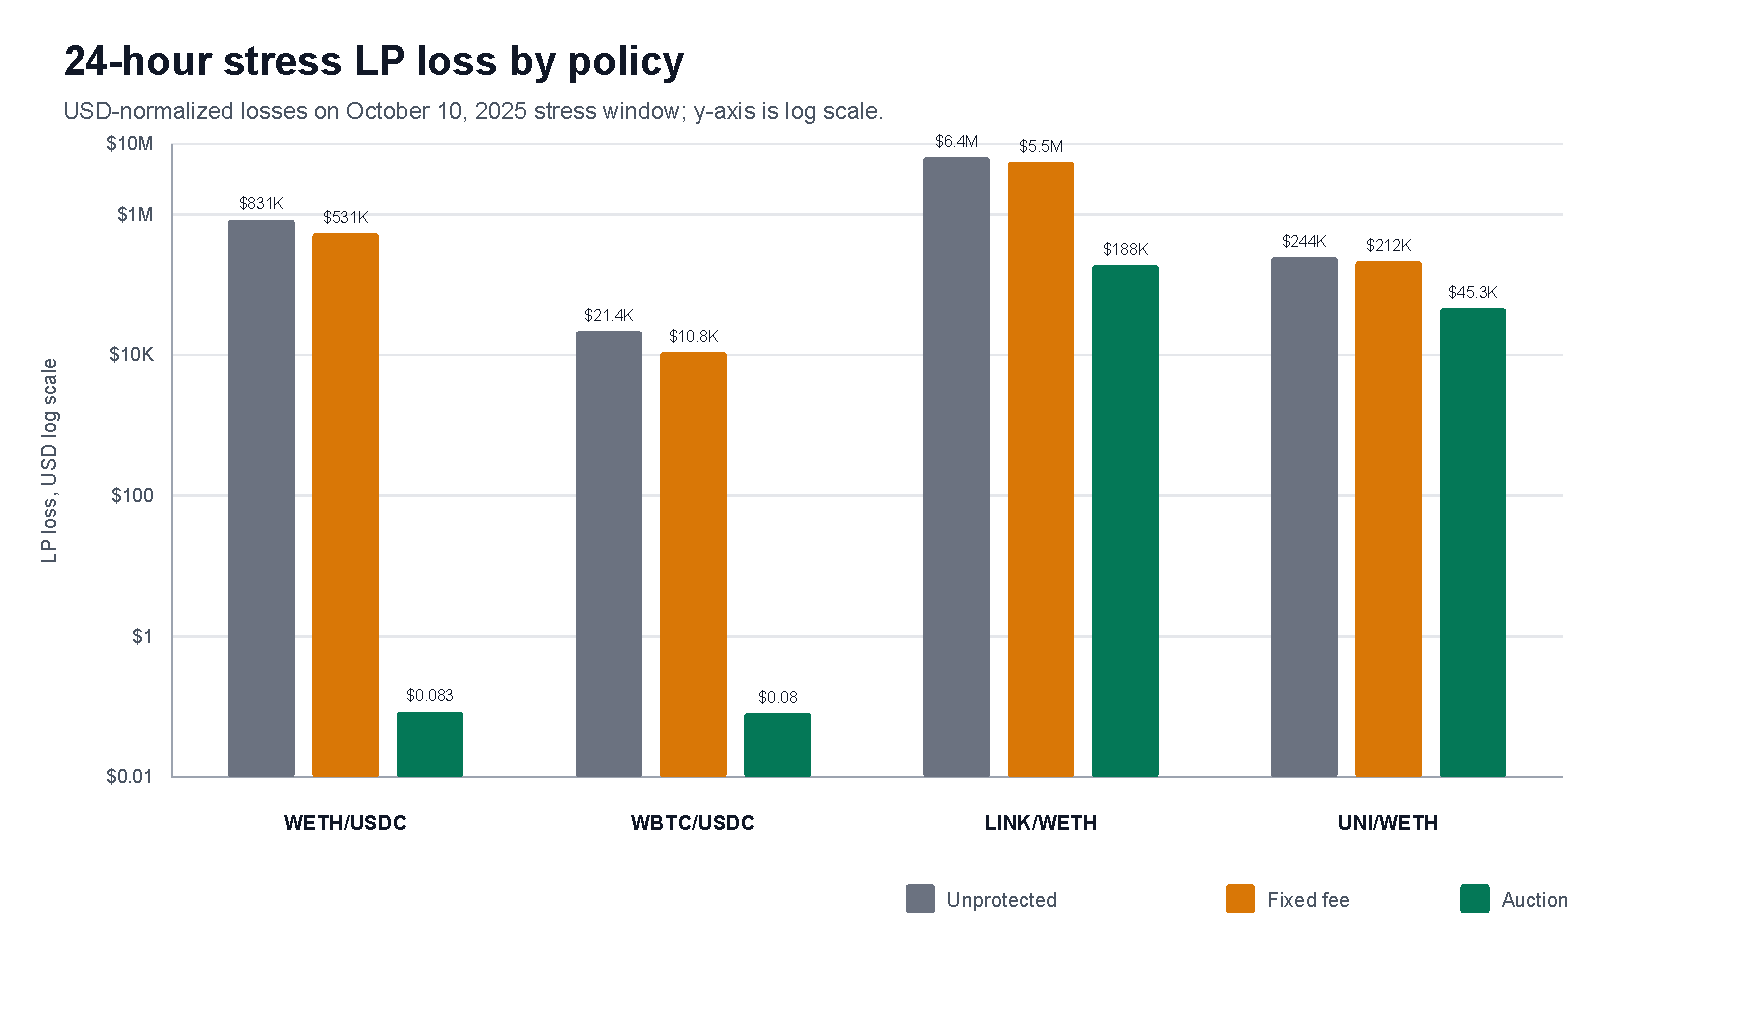
\includegraphics[width=\textwidth]{study_artifacts/month_2025_10_usd_floor/figures/stress_lp_loss_baselines_usd.pdf}
\caption{USD-normalized 24-hour stress losses by policy. The log scale is used because the auction policy drives WETH/USDC and WBTC/USDC residual LP loss below one dollar while LINK/WETH and UNI/WETH remain economically visible but still far below the unprotected and fixed-fee baselines.}
\label{fig:stress-loss-baselines}
\end{figure}

\subsection{Checkpointed October month and launch rule}

The checkpointed October run is the first month-scale artifact in this draft. It completed all 124 planned pool windows: 31 windows for each of WETH/USDC, WBTC/USDC, LINK/WETH, and UNI/WETH. The completed export covers 89,220 swap samples and 8,784 oracle updates. Table~\ref{tab:month-mixed-flow} reports the hook replay market-quality diagnostics. Executed benign flow pays no extra hook overcharge in these windows. The primary usability cost appears as rejected volume on the two USDC-quoted pools: WETH/USDC preserves 91.02\% of replay volume and WBTC/USDC preserves 89.55\%, with 72 and 84 stale-oracle rejections respectively. LINK/WETH and UNI/WETH preserve all replay volume in the checkpointed run.

\begin{table}[t]
\centering
\tiny
\resizebox{\textwidth}{!}{%
\begin{tabular}{@{}lrrrrrrrrrrr@{}}
\toprule
pool & completed windows & manifest windows & coverage pct & swaps & oracle updates & hook volume loss pct & hook volume preserved pct & hook benign extra cost bps & hook toxic clip pct & hook stale oracle rejects & hook fee cap rejects \\
\midrule
WETH/USDC 0.30\% & 31 & 31 & 100.00 & 25726 & 1415 & 8.9792 & 91.0208 & 0 & 0 & 72 & 0 \\
WBTC/USDC 0.05\% & 31 & 31 & 100.00 & 41861 & 999 & 10.4465 & 89.5535 & 0 & 0 & 84 & 0 \\
LINK/WETH 0.30\% & 31 & 31 & 100.00 & 14786 & 3779 & 0 & 100.00 & 0 & 0 & 0 & 0 \\
UNI/WETH 0.30\% & 31 & 31 & 100.00 & 6847 & 2591 & 0 & 100.00 & 0 & 0 & 0 & 0 \\
\bottomrule
\end{tabular}}
\caption{Checkpointed October 2025 mixed-flow usability summary. Coverage is the share of manifest windows currently exported for each pool.}
\label{tab:month-mixed-flow}
\end{table}


Table~\ref{tab:month-launch-policy-by-pool} reports selected launch rules from the 5,208-row USD-floor month sweep. The grid result is a unit-normalization lesson: when a positive stale-loss floor is used, it should be expressed in a common numeraire and converted to quote units per pool/window. A prior native-floor diagnostic showed why this matters: a 0.5 native-quote floor barely changes the two USDC pools, but under-triggers WETH-quoted LINK and UNI because 0.5 WETH is a much larger economic threshold.

The USD-floor rerun resolves the unit issue. With a \$0.50 floor and zero oracle-volatility threshold, WETH/USDC and WBTC/USDC remain at 91.82\% and 92.06\% recapture. LINK/WETH improves from 73.14\% under a 0.5 WETH floor to 99.92\%, and UNI/WETH improves from 35.60\% to 99.83\%, because the median native WETH floor is about 0.000124 WETH. Raising the oracle-volatility trigger to 25 bps remains acceptable for LINK and UNI but costs material recapture on WETH and WBTC; a 100 bps trigger is too conservative across all four pools.

\begin{figure}[H]
\centering
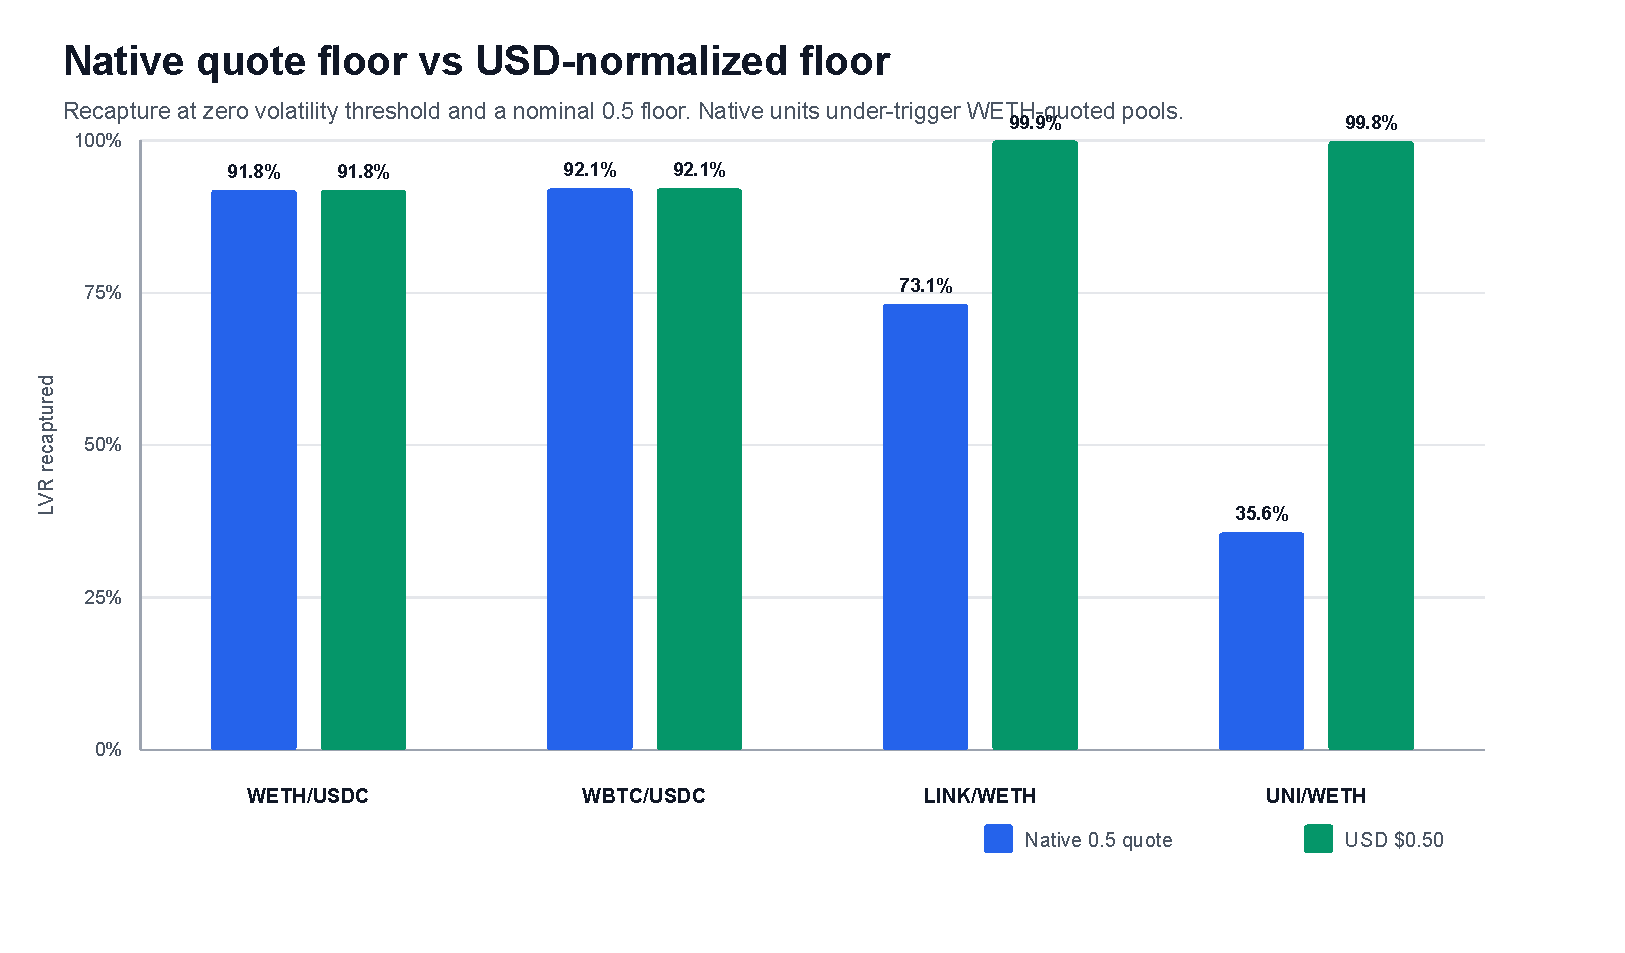
\includegraphics[width=0.92\textwidth]{study_artifacts/month_2025_10_usd_floor/figures/native_vs_usd_floor_recapture.pdf}
\caption{Native quote floors are not portable across quote assets. A 0.5 native-quote floor is approximately \$0.50 on USDC-quoted pools but roughly 0.5 WETH on WETH-quoted pools, causing LINK/WETH and UNI/WETH to under-trigger. Expressing the floor in USD restores trigger coverage without changing the USDC pools.}
\label{fig:native-vs-usd-floor}
\end{figure}

\begin{figure}[H]
\centering
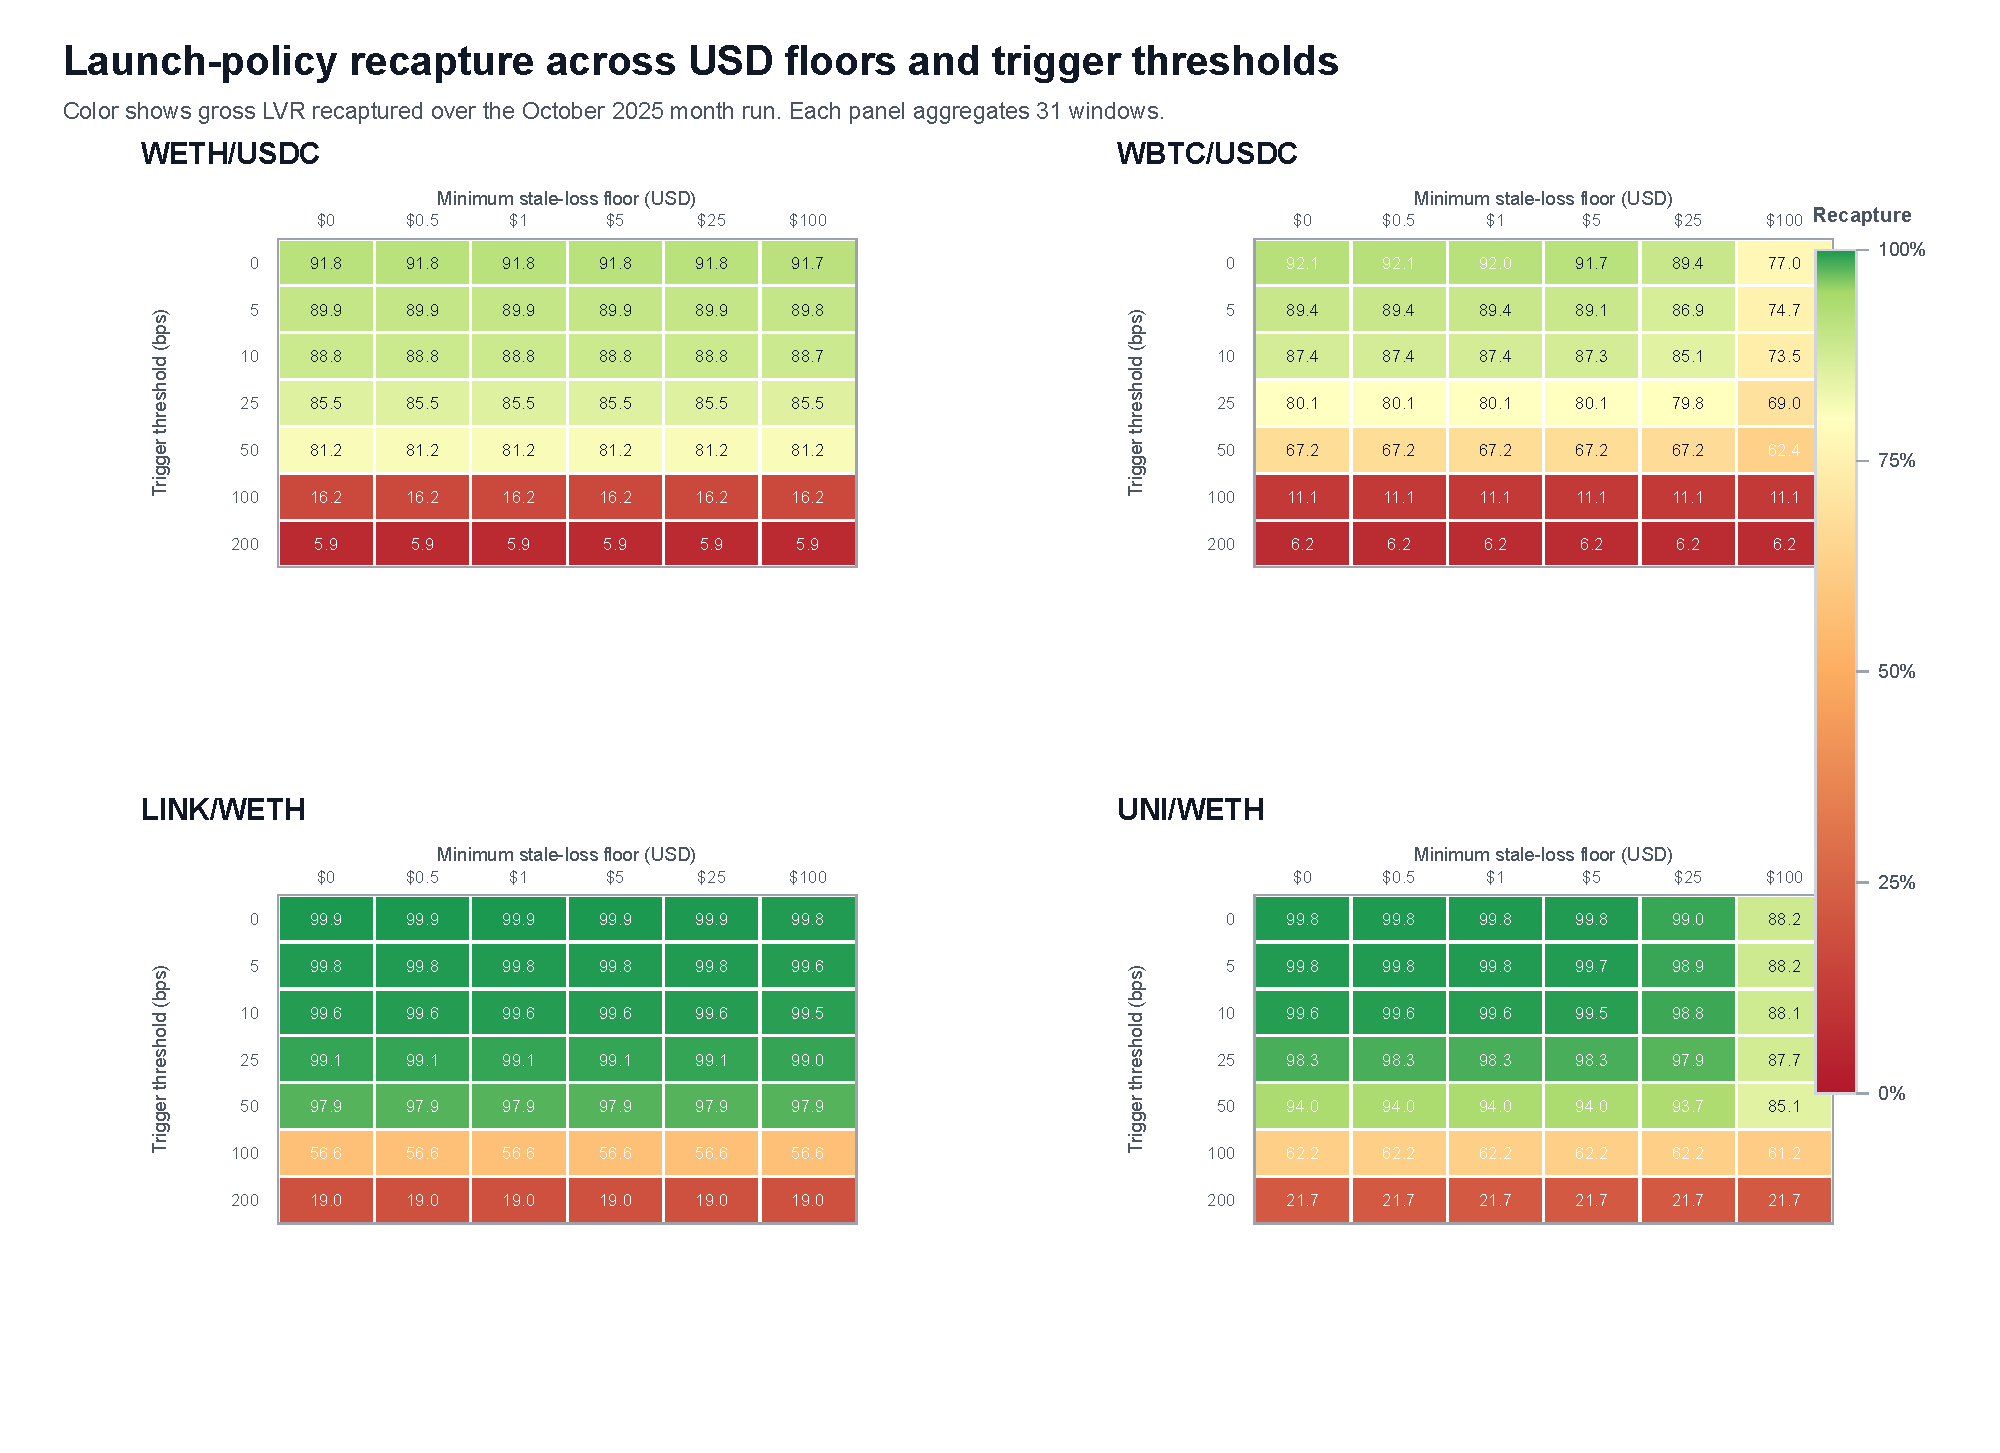
\includegraphics[width=\textwidth]{study_artifacts/month_2025_10_usd_floor/figures/launch_policy_heatmap.pdf}
\caption{Launch-policy sensitivity over USD stale-loss floors and oracle-volatility thresholds. The strongest month-scale policies launch immediately or at very low volatility thresholds. High trigger thresholds reduce recapture sharply, especially on the USDC-quoted pools.}
\label{fig:launch-policy-heatmap}
\end{figure}

A separate launch-rule correlation matrix is intentionally omitted: after month aggregation, reprice, no-trade, and fail-closed outcomes are constant, so their correlations are undefined and the figure adds visual noise rather than evidence. Figure~\ref{fig:launch-policy-heatmap} and Table~\ref{tab:month-launch-policy-by-pool} are the defensible launch-rule diagnostics.

\begin{table}[t]
\centering
\tiny
\resizebox{\textwidth}{!}{%
\begin{tabular}{@{}lrrrrrrrrrrrrrr@{}}
\toprule
pool & floor mode & oracle volatility threshold bps & min stale loss usd & median min stale loss quote & processed windows & recapture pct & trigger count & clear count & trade count & clear rate pct & reprice execution pct & no trade pct & fail closed pct & better windows \\
\midrule
WETH/USDC 0.30\% & usd & 0 & 0 & 0 & 31 & 91.8235 & 1357 & 1357 & 1393 & 100.00 & 100.00 & 8.9646 & 8.9646 & 31 \\
WETH/USDC 0.30\% & usd & 0 & 0.5 & 0.50007 & 31 & 91.8234 & 1331 & 1331 & 1393 & 100.00 & 100.00 & 8.9646 & 8.9646 & 31 \\
WETH/USDC 0.30\% & usd & 5.0000 & 0.5 & 0.50007 & 31 & 89.9017 & 1243 & 1243 & 1393 & 100.00 & 100.00 & 8.9646 & 8.9646 & 31 \\
WETH/USDC 0.30\% & usd & 25.0000 & 0.5 & 0.50007 & 31 & 85.4839 & 1010 & 1010 & 1393 & 100.00 & 100.00 & 8.9646 & 8.9646 & 31 \\
WETH/USDC 0.30\% & usd & 100.00 & 0.5 & 0.50007 & 31 & 16.1799 & 30 & 30 & 1393 & 100.00 & 100.00 & 8.9646 & 8.9646 & 1 \\
WBTC/USDC 0.05\% & usd & 0 & 0 & 0 & 31 & 92.0701 & 947 & 947 & 983 & 100.00 & 100.00 & 9.7942 & 9.7942 & 31 \\
WBTC/USDC 0.05\% & usd & 0 & 0.5 & 0.50007 & 31 & 92.0599 & 880 & 880 & 983 & 100.00 & 100.00 & 9.7942 & 9.7942 & 31 \\
WBTC/USDC 0.05\% & usd & 5.0000 & 0.5 & 0.50007 & 31 & 89.3940 & 830 & 830 & 983 & 100.00 & 100.00 & 9.7942 & 9.7942 & 31 \\
WBTC/USDC 0.05\% & usd & 25.0000 & 0.5 & 0.50007 & 31 & 80.0701 & 535 & 535 & 983 & 100.00 & 100.00 & 9.7942 & 9.7942 & 29 \\
WBTC/USDC 0.05\% & usd & 100.00 & 0.5 & 0.50007 & 31 & 11.1252 & 13 & 13 & 983 & 100.00 & 100.00 & 9.7942 & 9.7942 & 1 \\
LINK/WETH 0.30\% & usd & 0 & 0 & 0 & 31 & 99.9181 & 3467 & 3467 & 3485 & 100.00 & 100.00 & 0 & 0 & 31 \\
LINK/WETH 0.30\% & usd & 0 & 0.5 & 0.000124 & 31 & 99.9180 & 3418 & 3418 & 3485 & 100.00 & 100.00 & 0 & 0 & 31 \\
LINK/WETH 0.30\% & usd & 5.0000 & 0.5 & 0.000124 & 31 & 99.7896 & 3320 & 3320 & 3485 & 100.00 & 100.00 & 0 & 0 & 31 \\
LINK/WETH 0.30\% & usd & 25.0000 & 0.5 & 0.000124 & 31 & 99.0862 & 2959 & 2959 & 3485 & 100.00 & 100.00 & 0 & 0 & 31 \\
LINK/WETH 0.30\% & usd & 100.00 & 0.5 & 0.000124 & 31 & 56.5857 & 75 & 75 & 3485 & 100.00 & 100.00 & 0 & 0 & 1 \\
UNI/WETH 0.30\% & usd & 0 & 0 & 0 & 31 & 99.8340 & 2412 & 2412 & 2431 & 100.00 & 100.00 & 0 & 0 & 31 \\
UNI/WETH 0.30\% & usd & 0 & 0.5 & 0.000125 & 31 & 99.8307 & 2311 & 2311 & 2431 & 100.00 & 100.00 & 0 & 0 & 31 \\
UNI/WETH 0.30\% & usd & 5.0000 & 0.5 & 0.000125 & 31 & 99.7765 & 2278 & 2278 & 2431 & 100.00 & 100.00 & 0 & 0 & 31 \\
UNI/WETH 0.30\% & usd & 25.0000 & 0.5 & 0.000125 & 31 & 98.3351 & 1902 & 1902 & 2431 & 100.00 & 100.00 & 0 & 0 & 31 \\
UNI/WETH 0.30\% & usd & 100.00 & 0.5 & 0.000125 & 31 & 62.1995 & 454 & 454 & 2431 & 100.00 & 100.00 & 0 & 0 & 27 \\
\bottomrule
\end{tabular}}
\caption{Selected October 2025 Dutch-auction launch rules by pool. Recapture and execution columns are dimensionless, avoiding cross-pool native-quote aggregation.}
\label{tab:month-launch-policy-by-pool}
\end{table}


The aggregate top-policy table is retained as an artifact in \path{study_artifacts/month_2025_10_usd_floor/month_launch_policy_top.csv}, but it mixes USDC- and WETH-denominated quote values. It should be used only as a ranking diagnostic, not as a cross-pool welfare total. A WBTC/USDC unit audit in \path{study_artifacts/month_2025_10_usd_floor/wbtc_quote_unit_audit.md} confirms that the month launch-policy outputs are decimal-normalized human USDC units; the older observed-flow \texttt{dutch\_auction\_lp\_net\_quote} window-summary field remains excluded from publication totals.

\subsection{Auction robustness sweep}

Table~\ref{tab:robustness} reports the completed 1,024-row sweep over \texttt{base\_fee\_bps}, \texttt{alpha\_bps}, maximum concession, solver gas, solver edge, auction duration, reserve margin, and \texttt{min\_stale\_loss\_quote}. The sweep covers the first six hours of the saved October 10 stress day. The classification rule labels a configuration better only when the bootstrap lower confidence bound for LP uplift is positive and mean delay remains within the five-block budget.

\begin{table}[t]
\centering
\tiny
\resizebox{\textwidth}{!}{%
\begin{tabular}{@{}l r r r r r r r@{}}
\toprule
Policy & \shortstack{LP loss\\quote} & \shortstack{Uplift vs\\unprotected} & Recapture & Reprice & Stale & No-trade & Clear \\
\midrule
No auction & 9{,}458.88 & -- & 0.00\% & 100.00\% & 0.00\% & 0.00\% & 0.00\% \\
Fixed fee & 41.00 & -- & 98.4783\% & 3.5076\% & 84.5212\% & 82.7160\% & 0.00\% \\
Auction, execution constrained & 0.000946 & 9{,}458.88 & 99.99999\% & 100.00\% & 0.00\% & 0.00\% & 100.00\% \\
LP-only best, stale control & 0.00 & 9{,}458.88 & -- & 0.00\% & 100.00\% & 100.00\% & 0.00\% \\
\bottomrule
\end{tabular}}
\caption{Robustness sweep summary. The LP-only optimum is a degenerate no-trade/stale policy, so execution-constrained selection is the relevant design objective. Across the 1,024 configurations, 416 were classified better, 608 neutral, and 0 worse under the exploratory bootstrap rule.}
\label{tab:robustness}
\end{table}

The sweep turns an earlier planned robustness item into a stronger design constraint: optimizing LP net alone can select a policy that simply never reprices. A publishable version should therefore rank policies by LP outcome subject to explicit execution, delay, and stale-time constraints.

Figure~\ref{fig:dutch-auction-correlations} is descriptive rather than causal, but it is useful for policy selection. It shows that unconstrained LP optimization can reward stale control: higher \texttt{alpha\_bps} improves measured LP uplift while suppressing repricing and increasing no-trade and stale-time shares. The production interpretation is therefore not ``maximize alpha.'' It is to choose auction parameters under explicit liveness constraints. The same matrix also shows that solver gas and solver edge are the main market-quality frictions in this sweep, reducing recapture, clear rates, and the probability that a configuration beats the baseline. By contrast, start concession, concession growth, quote floor, maximum concession, duration, and reserve margin are weak drivers over this tested grid.

\begin{center}
\centering
\makebox[\textwidth][c]{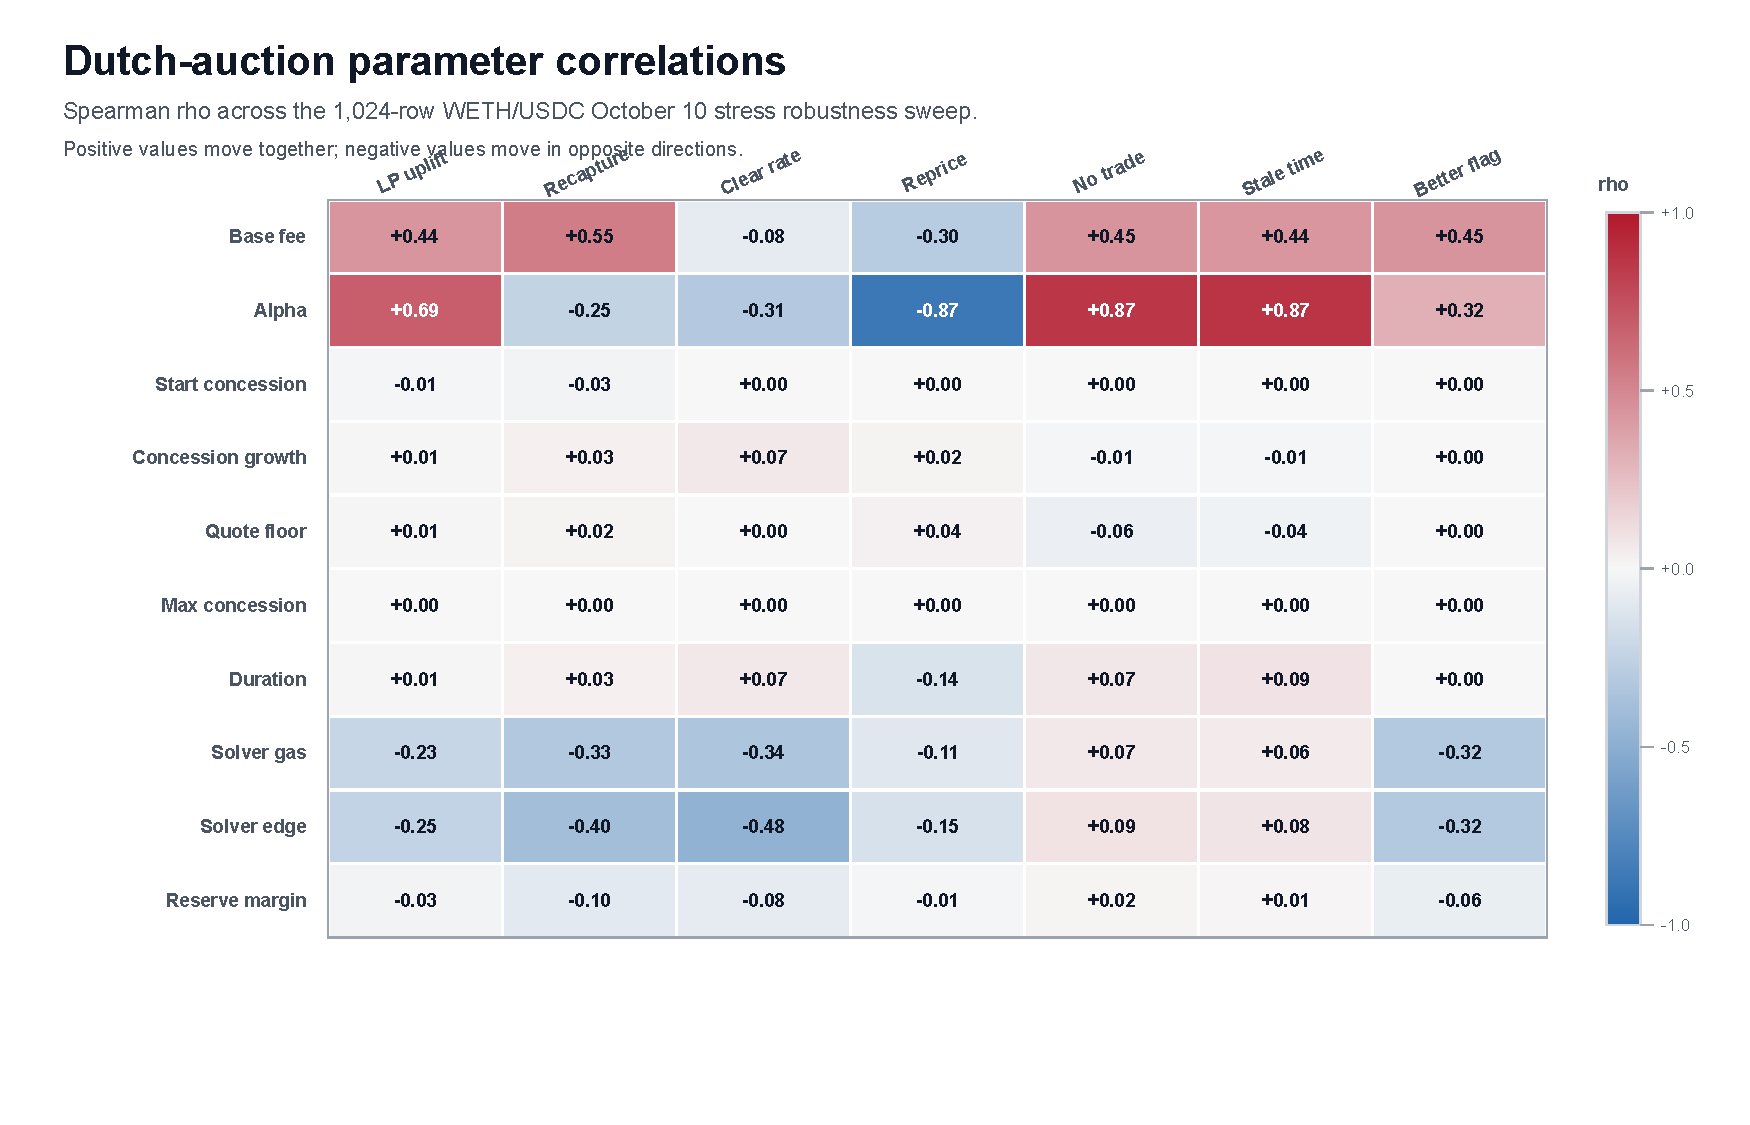
\includegraphics[width=0.94\textwidth]{study_artifacts/month_2025_10_usd_floor/figures/dutch_auction_parameter_correlations.pdf}}
\parbox{0.94\textwidth}{\refstepcounter{figure}\label{fig:dutch-auction-correlations}\small\textbf{Figure~\thefigure.} Spearman rank correlations between Dutch-auction parameters and robustness-sweep outcomes. Higher \texttt{alpha\_bps} correlates positively with LP uplift but also strongly with no-trade and stale time and negatively with repricing, which identifies the stale-control failure mode. Solver gas and solver edge move against LP uplift, recapture, clear rate, and the ``better'' classification.}
\end{center}

\begin{table}[H]
\centering
\tiny
\resizebox{\textwidth}{!}{%
\begin{tabular}{@{}lrrrrrrrrrr@{}}
\toprule
Selection & base fee bps & alpha bps & min stale quote & solver gas quote & solver edge bps & recapture pct & reprice pct & no trade pct & stale pct & clear pct \\
\midrule
Execution constrained & 0 & 0 & 0.5 & 0 & 0 & 100.0000 & 100.00 & 0 & 0 & 100.00 \\
LP-only stale optimum & 5.0000 & 10,000.00 & 0.5 & 0 & 0 &  & 0 & 100.00 & 100.00 & 0 \\
LP net with delay budget & 0 & 10,000.00 & 0.5 & 0 & 0 & 100.0000 & 1.8665 & 38.2716 & 39.6993 & 100.00 \\
\bottomrule
\end{tabular}}
\caption{Parameter selections from the WETH/USDC six-hour Dutch-auction robustness sweep. The selected rows share a 0.001 bps start concession, zero concession growth, 5{,}000 bps max concession, zero-second duration, and zero reserve margin. The LP-only optimum is included as a negative-control warning because it maximizes LP net by leaving the pool stale rather than preserving repricing.}
\label{tab:dutch-auction-best-params}
\end{table}


\subsection{Multi-window and out-of-sample evidence}

The checkpointed October run above is the main scale-up beyond one day. Table~\ref{tab:multi-window} preserves the earlier replay-clean ablation as a diagnostic: it reports 44 exact-replay-clean normal/stress windows, plus quiet and volatile terciles formed by realized reference-price movement within the saved windows. The values are pool-native quote units; the cross-pool USD table is the appropriate place for cross-asset welfare comparisons.

\begin{table}[t]
\centering
\tiny
\resizebox{\textwidth}{!}{%
\begin{tabular}{@{}l r r r r r r r r@{}}
\toprule
Bucket & Windows & Swaps & Mean & Median & P05 & P95 & \shortstack{95\% CI\\low} & \shortstack{95\% CI\\high} \\
\midrule
All replay-clean windows & 44 & 7{,}019 & 3.4039 & 0.0000 & 0.0000 & 16.7692 & 1.8623 & 5.1406 \\
Normal windows & 30 & 6{,}149 & 3.6047 & 0.0000 & 0.0000 & 17.0614 & 1.6961 & 5.8142 \\
Stress/oracle-fail windows & 14 & 870 & 2.9735 & 0.2503 & 0.0000 & 15.0651 & 0.5519 & 5.8450 \\
Quiet realized-move tercile & 14 & 550 & 0.3113 & 0.0000 & 0.0000 & 1.9987 & 0.0000 & 0.7512 \\
Middle realized-move tercile & 16 & 1{,}817 & 1.1172 & 0.2503 & 0.0000 & 4.2286 & 0.4186 & 1.9980 \\
Volatile realized-move tercile & 14 & 4{,}652 & 9.1098 & 10.1091 & 0.0000 & 17.0744 & 5.5233 & 12.4136 \\
\bottomrule
\end{tabular}}
\caption{Multi-window LP uplift versus hook, in pool-native quote units. The confidence intervals are exploratory iid window bootstraps from the regenerated table.}
\label{tab:multi-window}
\end{table}

Held-out agent simulations provide additional support but should be treated as exploratory because the holdout set is small. The out-of-sample windows show auction losses near zero on held-out normal, stress, and DAI/USDC alternate-pool windows, but one normal holdout carries an overfit warning because the selected training configuration was weakly identified.

\begin{table}[t]
\centering
\tiny
\begin{tabular}{@{}l r r r r r l@{}}
\toprule
Window & \shortstack{Baseline\\loss} & \shortstack{Fixed-fee\\loss} & \shortstack{Auction\\loss} & Recapture & No-trade & Class \\
\midrule
holdout\_alt\_dai & 512.42 & 218.16 & 0.000051 & 99.99999\% & 55.56\% & better \\
holdout\_normal\_p01 & 1.0471 & 0.00 & 0.000000 & 99.99999\% & 21.43\% & better, overfit warning \\
holdout\_stress\_p02 & 1{,}057.06 & 0.00 & 0.000106 & 99.99999\% & 0.00\% & better \\
\bottomrule
\end{tabular}
\caption{Out-of-sample validation summary from the saved floor-optimization artifact. Quote units are pool-native.}
\label{tab:oos}
\end{table}

\section{Implementation Notes}

\paragraph{Oracle quality.}
The design assumes a trustworthy reference price. Production deployment should use high-quality oracles, explicit staleness checks, conservative maximum fee settings, and fail-closed behavior.

\paragraph{Launch thresholds.}
The month sweep shows that launch thresholds are unit-sensitive. A minimum stale-loss floor expressed in native quote units should not be shared across USDC- and WETH-quoted pools without normalization. The USD-floor rerun supports defining floors in a common numeraire, with per-window conversion to quote units from the quote feed.

\paragraph{Governance.}
The hook-only phase can use owner-managed configuration in a research setting. An auction module with external solver participation should put parameters behind a timelock and include emergency pause/cancel semantics.

\paragraph{No production auction claim.}
The current hook does not open or settle auctions on-chain. The interface and operational spec are sketches for the proposed module. The paper should not describe the auction path as deployed behavior.

\section{Conclusion}

The updated evidence supports a sharper thesis: low-LVR v4 pool design is not just dynamic fee control. The fee identity gives the correct stale-loss accounting; width and centering guards limit marginal-liquidity fragility; and auctioned repricing can preserve price discovery while redirecting most informed-flow surplus back to LPs. The October month run also sharpens the launch-rule design: a universal native-quote stale-loss floor is not portable across USDC- and WETH-quoted pools, while a USD-normalized floor restores LINK and UNI trigger coverage without disturbing the USDC pools. The main remaining research risk is no longer the fee identity. It is whether a production auction module can preserve the favorable adversarial-repricing results while improving mixed-flow liveness and volume preservation.

\begin{thebibliography}{10}

\bibitem{milionis-lvr}
Jason Milionis, Ciamac C. Moallemi, Tim Roughgarden, and Anthony Lee Zhang.
\newblock Automated Market Making and Loss-Versus-Rebalancing.
\newblock arXiv:2208.06046, revised May 2024.
\newblock \url{https://arxiv.org/abs/2208.06046}.

\bibitem{milionis-fees}
Jason Milionis, Ciamac C. Moallemi, and Tim Roughgarden.
\newblock Automated Market Making and Arbitrage Profits in the Presence of Fees.
\newblock arXiv:2305.14604, revised July 2025.
\newblock \url{https://arxiv.org/abs/2305.14604}.

\bibitem{uniswap-v4}
Hayden Adams, Moody Salem, Noah Zinsmeister, Sara Reynolds, Austin Adams, Will Pote, Mark Toda, Alice Henshaw, Emily Williams, and Dan Robinson.
\newblock Uniswap v4 Core Whitepaper.
\newblock August 2024.
\newblock \url{https://app.uniswap.org/whitepaper-v4.pdf}.

\bibitem{amamm}
Austin Adams, Ciamac C. Moallemi, Sara Reynolds, and Dan Robinson.
\newblock am-AMM: An Auction-Managed Automated Market Maker.
\newblock arXiv:2403.03367, 2024.
\newblock \url{https://arxiv.org/abs/2403.03367}.

\bibitem{baggiani-dynamic-fees}
Leonardo Baggiani, Martin Herdegen, and Leandro Sanchez-Betancourt.
\newblock Optimal Dynamic Fees in Automated Market Makers.
\newblock arXiv:2506.02869, 2025.
\newblock \url{https://arxiv.org/abs/2506.02869}.

\bibitem{budish-batch}
Eric Budish, Peter Cramton, and John Shim.
\newblock The High-Frequency Trading Arms Race: Frequent Batch Auctions as a Market Design Response.
\newblock \emph{The Quarterly Journal of Economics}, 130(4):1547--1621, 2015.
\newblock \url{https://doi.org/10.1093/qje/qjv027}.

\bibitem{uniswapx}
Hayden Adams, Noah Zinsmeister, Mark Toda, Emily Williams, Xin Wan, Matteo Leibowitz, Will Pote, Allen Lin, Eric Zhong, Zhiyuan Yang, Riley Campbell, Alex Karys, and Dan Robinson.
\newblock UniswapX.
\newblock July 2023.
\newblock \url{https://uniswap.org/whitepaper-uniswapx.pdf}.

\bibitem{cow-protocol}
CoW DAO.
\newblock CoW Protocol Documentation: Fair Combinatorial Batch Auction and Solvers.
\newblock \url{https://docs.cow.fi/}.

\bibitem{angeris-oracles}
Guillermo Angeris and Tarun Chitra.
\newblock Improved Price Oracles: Constant Function Market Makers.
\newblock arXiv:2003.10001, 2020.
\newblock \url{https://arxiv.org/abs/2003.10001}.

\bibitem{dodo-pmm}
DODO.
\newblock PMM Algorithm Documentation.
\newblock \url{https://docs.dodoex.io/en/product/pmm-algorithm}.

\end{thebibliography}

\end{document}
